\documentclass[10pt]{beamer}
\usetheme[
%%% option passed to the outer theme
%    progressstyle=fixedCircCnt,   % fixedCircCnt, movingCircCnt (moving is deault)
  ]{Feather}

% If you want to change the colors of the various elements in the theme, edit and uncomment the following lines

% Change the bar colors:
%\setbeamercolor{Feather}{fg=red!20,bg=red}

% Change the color of the structural elements:
%\setbeamercolor{structure}{fg=red}

% Change the frame title text color:
%\setbeamercolor{frametitle}{fg=blue}

% Change the normal text color background:
%\setbeamercolor{normal text}{fg=black,bg=gray!10}

%-------------------------------------------------------
% INCLUDE PACKAGES
%-------------------------------------------------------

\usepackage[utf8]{inputenc}
\usepackage[english]{babel}
\usepackage[T1]{fontenc}
\usepackage{helvet}
\usepackage{listings}

%-------------------------------------------------------
% DEFFINING AND REDEFINING COMMANDS
%-------------------------------------------------------

% colored hyperlinks
\newcommand{\chref}[2]{
  \href{#1}{{\usebeamercolor[bg]{Feather}#2}}
}

%-------------------------------------------------------
% Configure syntax highlight
%-------------------------------------------------------
\lstset{
  backgroundcolor=\color{white},
  breaklines=true,
  commentstyle=\color{green},
  extendedchars=true,
  frame=single,
  keepspaces=true,
  keywordstyle=\color{blue},
  language=Ruby,
  numbers=left,
  numbersep=10pt,
  numberstyle=\small\color{gray},
  rulecolor=\color{black},
  stringstyle=\color{blue},
  tabsize=2
}

%-------------------------------------------------------
% INFORMATION IN THE TITLE PAGE
%-------------------------------------------------------

\title[] % [] is optional - is placed on the bottom of the sidebar on every slide
{ % is placed on the title page
      \textbf{Vagrant}
}

\subtitle[Vagrant]
{
}

\author[Rodrigo Siqueira Jordão]
{      Rodrigo Siqueira Jordão \\
      {\ttfamily siqueira@kuniri.org}
}

\institute[]
{
      Institute of Mathematics and Statistics\\
      University of Sao Paulo\\

  %there must be an empty line above this line - otherwise some unwanted space
  % is added between the university and the country (I do not know why;( )
}

\date{\today}

%-------------------------------------------------------
% THE BODY OF THE PRESENTATION
%-------------------------------------------------------

\begin{document}

%-------------------------------------------------------
% THE TITLEPAGE
%-------------------------------------------------------

{\1% % this is the name of the PDF file for the background
% the plain option removes the header from the title page, noframenumbering removes the numbering of this frame only
\begin{frame}[plain,noframenumbering]
  \titlepage % call the title page information from above
\end{frame}}

\begin{frame}[shrink]{Content}{}
  \tableofcontents
\end{frame}

%=======================================================
\section{Introduction}
%=======================================================
\begin{frame}{Introduction}{What is vagrant?}
  \begin{columns}[T]

    \begin{column}{.6\textwidth}
      \begin{itemize}
        \item Creates and configures virtual development
        \item Wrapper around virtualization
      \end{itemize}
    \end{column}

    \hfill

    \begin{column}{.4\textwidth}
      \centering
      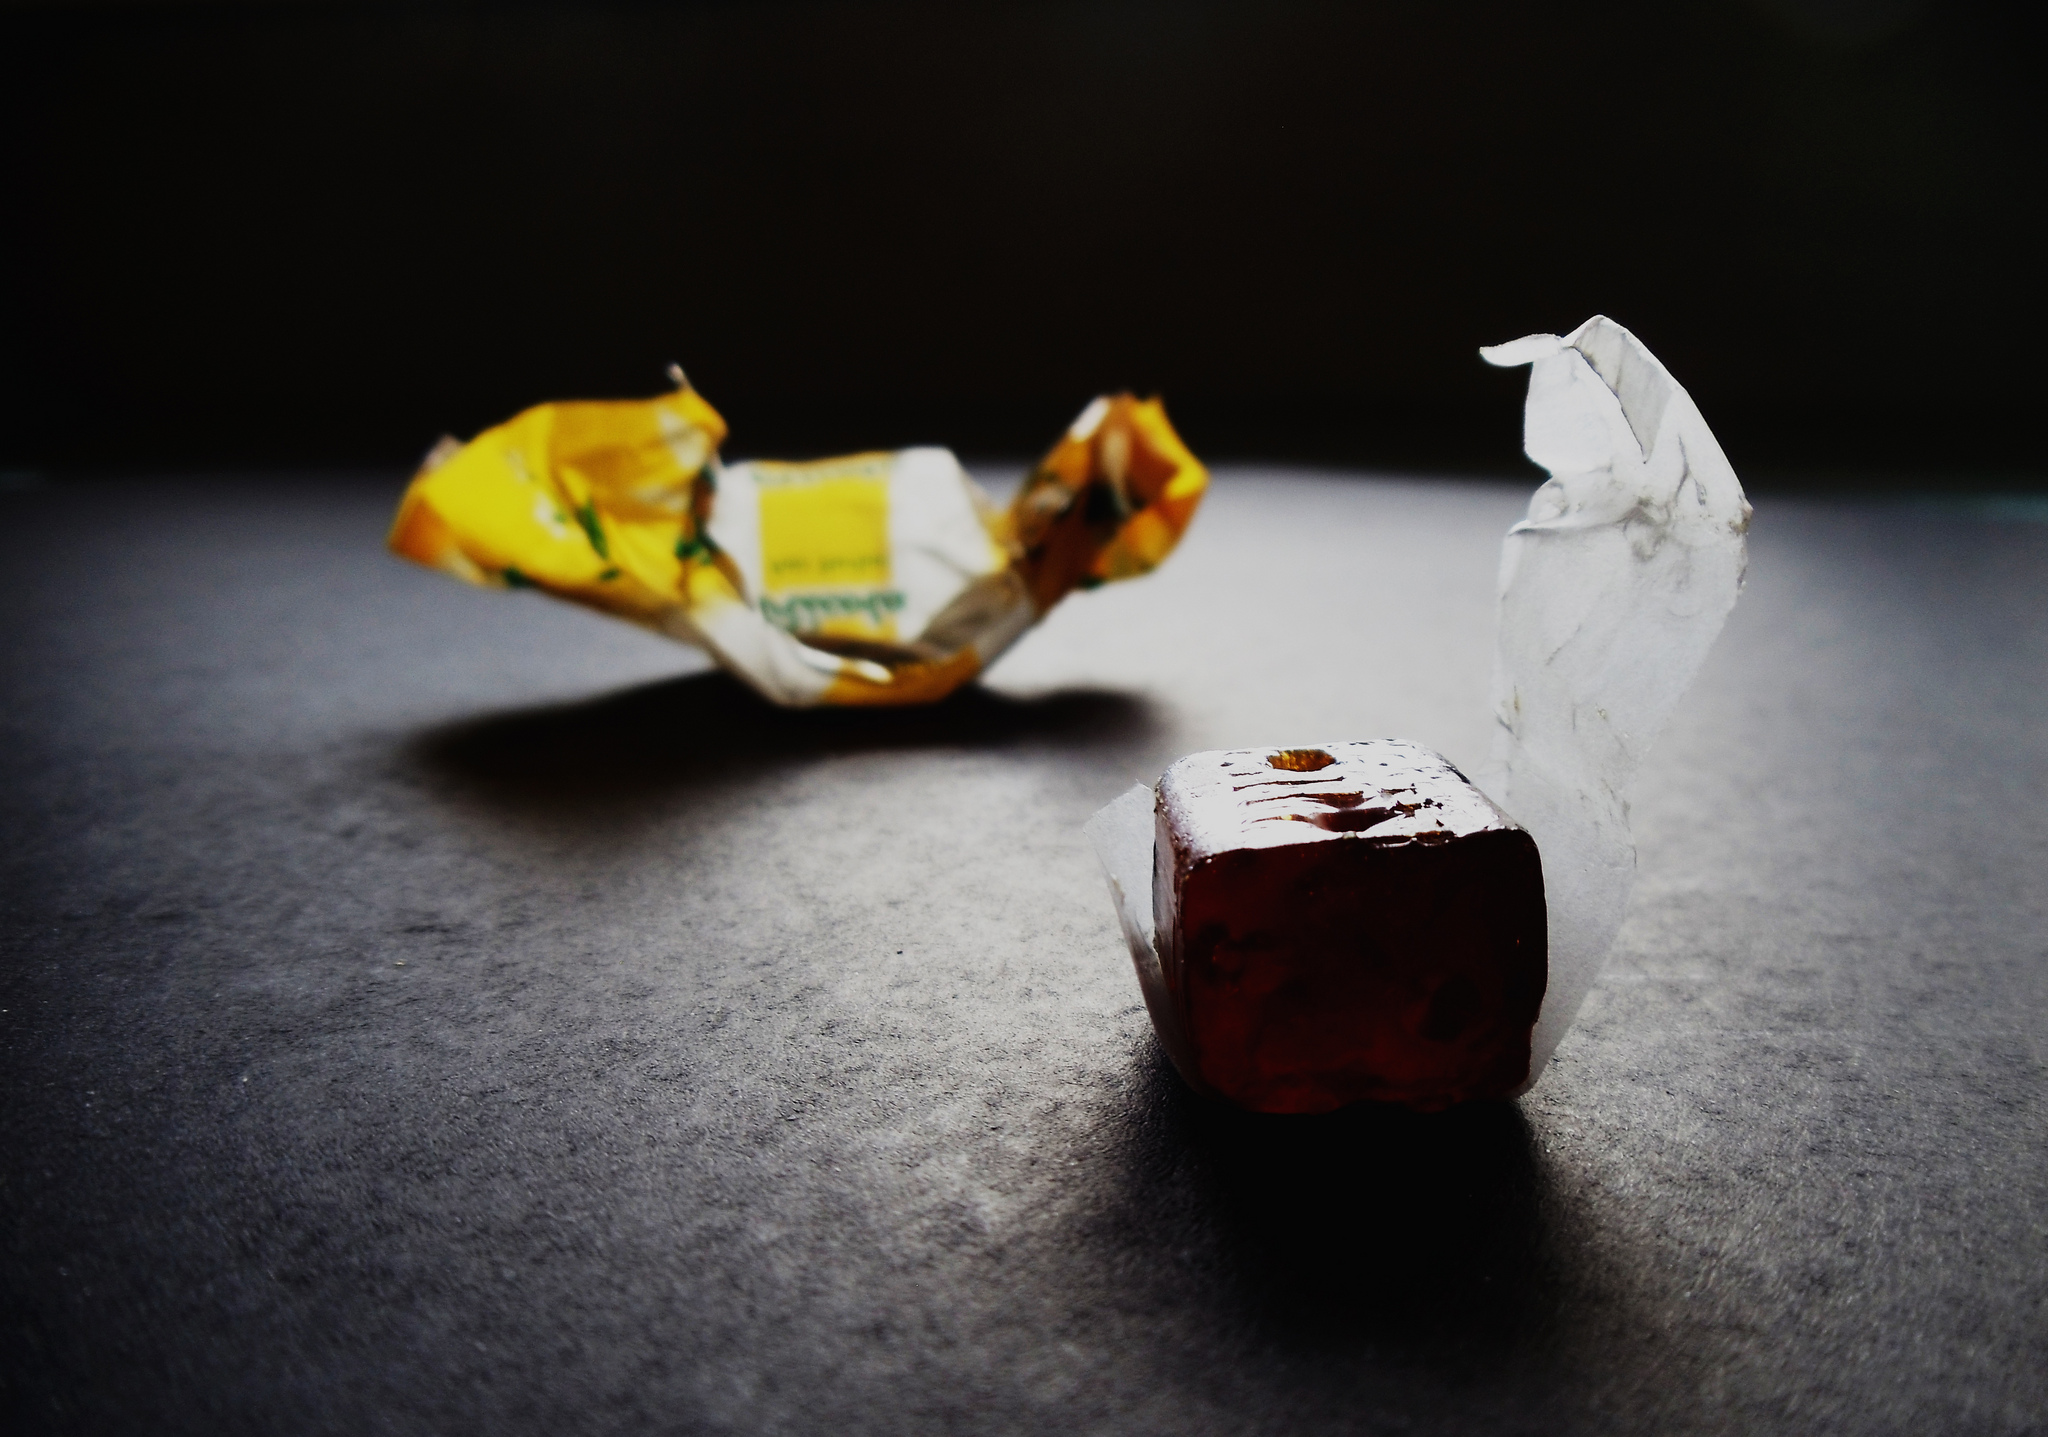
\includegraphics[width=1\textwidth, keepaspectratio=true]{images/wrapper.jpg}
    \end{column}
  \end{columns}
\end{frame}

\begin{frame}{Features}{Say goodbye to "works on my machine" bugs}
  \begin{columns}[T]

    \begin{column}{.7\textwidth}
      \begin{itemize}
        \item Isolate dependencies and their configuration
        \item Consistent environment
        \item Simple to other people replicate the same environment
        \item virtualization supported by vagrant:
          \begin{itemize}
            \item VirtualBox
            \item VMware
            \item KVM
            \item Linux Containers (LXC)
          \end{itemize}
      \end{itemize}
    \end{column}

    \hfill

    \begin{column}{.3\textwidth}
      \centering
      
\includegraphics[width=1\textwidth, keepaspectratio=true]{images/vagrant.png}
    \end{column}
  \end{columns}
\end{frame}

%=======================================================
\section{Let's start to work}
%=======================================================

\begin{frame}{Let's start to work}{Let's start to work}
  
\includegraphics[width=1\textwidth, keepaspectratio=true]{images/work.jpg}
\end{frame}

\begin{frame}[fragile]{Let's start to work}{Create and wake up your vm}
\begin{lstlisting}
vagrant init hashicorp/precise64
\end{lstlisting}

Vagrant file will be generated (look at the Vagrant file generated)
\pause

\begin{lstlisting}
vagrant up
vagrant up --provider virtualbox
\end{lstlisting}
Start running VM

\end{frame}

\begin{frame}[fragile]{Let's start to work}{Enter in your vm}
\begin{lstlisting}
vagrant ssh
\end{lstlisting}
Just do whatever you want :)
\end{frame}

\begin{frame}[fragile]{Let's start to work}{Pack and unpack your image}

Do you want to take a snapshot of your vm? Easy...

\begin{lstlisting}
vagrant package --output weS2opensource.box
\end{lstlisting}

\pause

Unpack

\begin{lstlisting}
vagrant box add opensourceLife weS2opensource.box
vagrant box list
\end{lstlisting}

\end{frame}

\begin{frame}[fragile]{Let's start to work}{Destroy your vm}
\begin{lstlisting}
vagrant global-status
vagrant destroy <id>
\end{lstlisting}
Just do whatever you want :)
\end{frame}

%=======================================================
\section{Improve your provision}
%=======================================================

\begin{frame}[fragile]{Improve our Vagrantfile}{provision}

If you want to add provision, follow the code below:

\begin{lstlisting}
httpd.vm.provision 'shell', privileged: true,
         keep_color: true,
         path: 'vagrant/bootstrap.sh'
\end{lstlisting}

\pause
Creating an bridge
\begin{lstlisting}
httpd.vm.network 'forwarded_port',
					guest: 80, host: 8080
\end{lstlisting}

\end{frame}

{\1
\begin{frame}[plain,noframenumbering]
  \finalpage{Thank you!}
\end{frame}}

\end{document}
